\section{Overview of Results}

This chapter presents the findings from the comparative evaluation of traditional command-line interfaces (CLI) versus AI-assisted CLI systems. The analysis is based on experimental data collected through controlled user testing sessions, examining key performance metrics including task completion time, success rates, number of attempts, and user satisfaction ratings across ease of use, confidence, and frustration dimensions.

\section{Quantitative Results}

The quantitative analysis focuses on measurable performance indicators that directly assess the effectiveness of AI-assisted CLI in comparison to traditional CLI methods. These metrics provide objective evidence for the impact of AI integration on user productivity and task completion efficiency.

\subsection{Task Completion Time Analysis}

Analysis of task completion times reveals substantial performance improvements with AI assistance, with an overall 40\% reduction in average completion time (97.7s traditional vs 58.9s AI-assisted). The improvements vary significantly by task category:

\begin{itemize}
	\item \textbf{File viewing:} Most dramatic improvement with 90\% time reduction (228s vs 22s average)
	\item \textbf{File management:} 43\% improvement (79.6s vs 45.0s average)
	\item \textbf{File navigation:} 40\% improvement (99.6s vs 59.4s average)
\end{itemize}

Categories exclusively performed with AI assistance (File search, Text search, Text processing) showed completion times ranging from 21.7s to 120.4s, indicating effective AI support for complex operations. The data demonstrates that AI assistance provides the greatest benefit for tasks requiring specific syntax knowledge or complex command structures.

Table~\ref{tab:results_summary} presents a preliminary summary of the key performance metrics across both interface conditions:

\begin{table}[h]
	\centering
	\caption{Performance Comparison Summary}
	\label{tab:results_summary}
	\begin{tabular}{|l|c|c|c|}
		\hline
		\textbf{Metric}             & \textbf{Traditional CLI} & \textbf{AI-Assisted CLI} & \textbf{Improvement} \\
		\hline
		Average Task Time (seconds) & 97.7                     & 58.9                     & 40\%                 \\
		\hline
		Success Rate (\%)           & 84.6                     & 97.5                     & 15\%                 \\
		\hline
		Average Attempts per Task   & 2.38                     & 1.43                     & 40\%                 \\
		\hline
		Ease of Use Rating (1-5)    & N/A                      & 4.83                     & Favors AI            \\
		\hline
		Confidence Rating (1-5)     & N/A                      & 3.83                     & Favors AI            \\
		\hline
		Frustration Rating (1-5)    & N/A                      & 2.17                     & Less frustrating     \\
		\hline
	\end{tabular}
\end{table}

The results demonstrate consistent improvements across all measured dimensions when AI assistance is available. AI-assisted CLI shows a 40\% reduction in task completion time, 15\% improvement in success rate, and 40\% reduction in average attempts per task compared to traditional CLI.

Figure~\ref{fig:performance_comparison} provides a comprehensive overview of the key performance metrics across both interface conditions.

\begin{figure}[h]
	\centering
	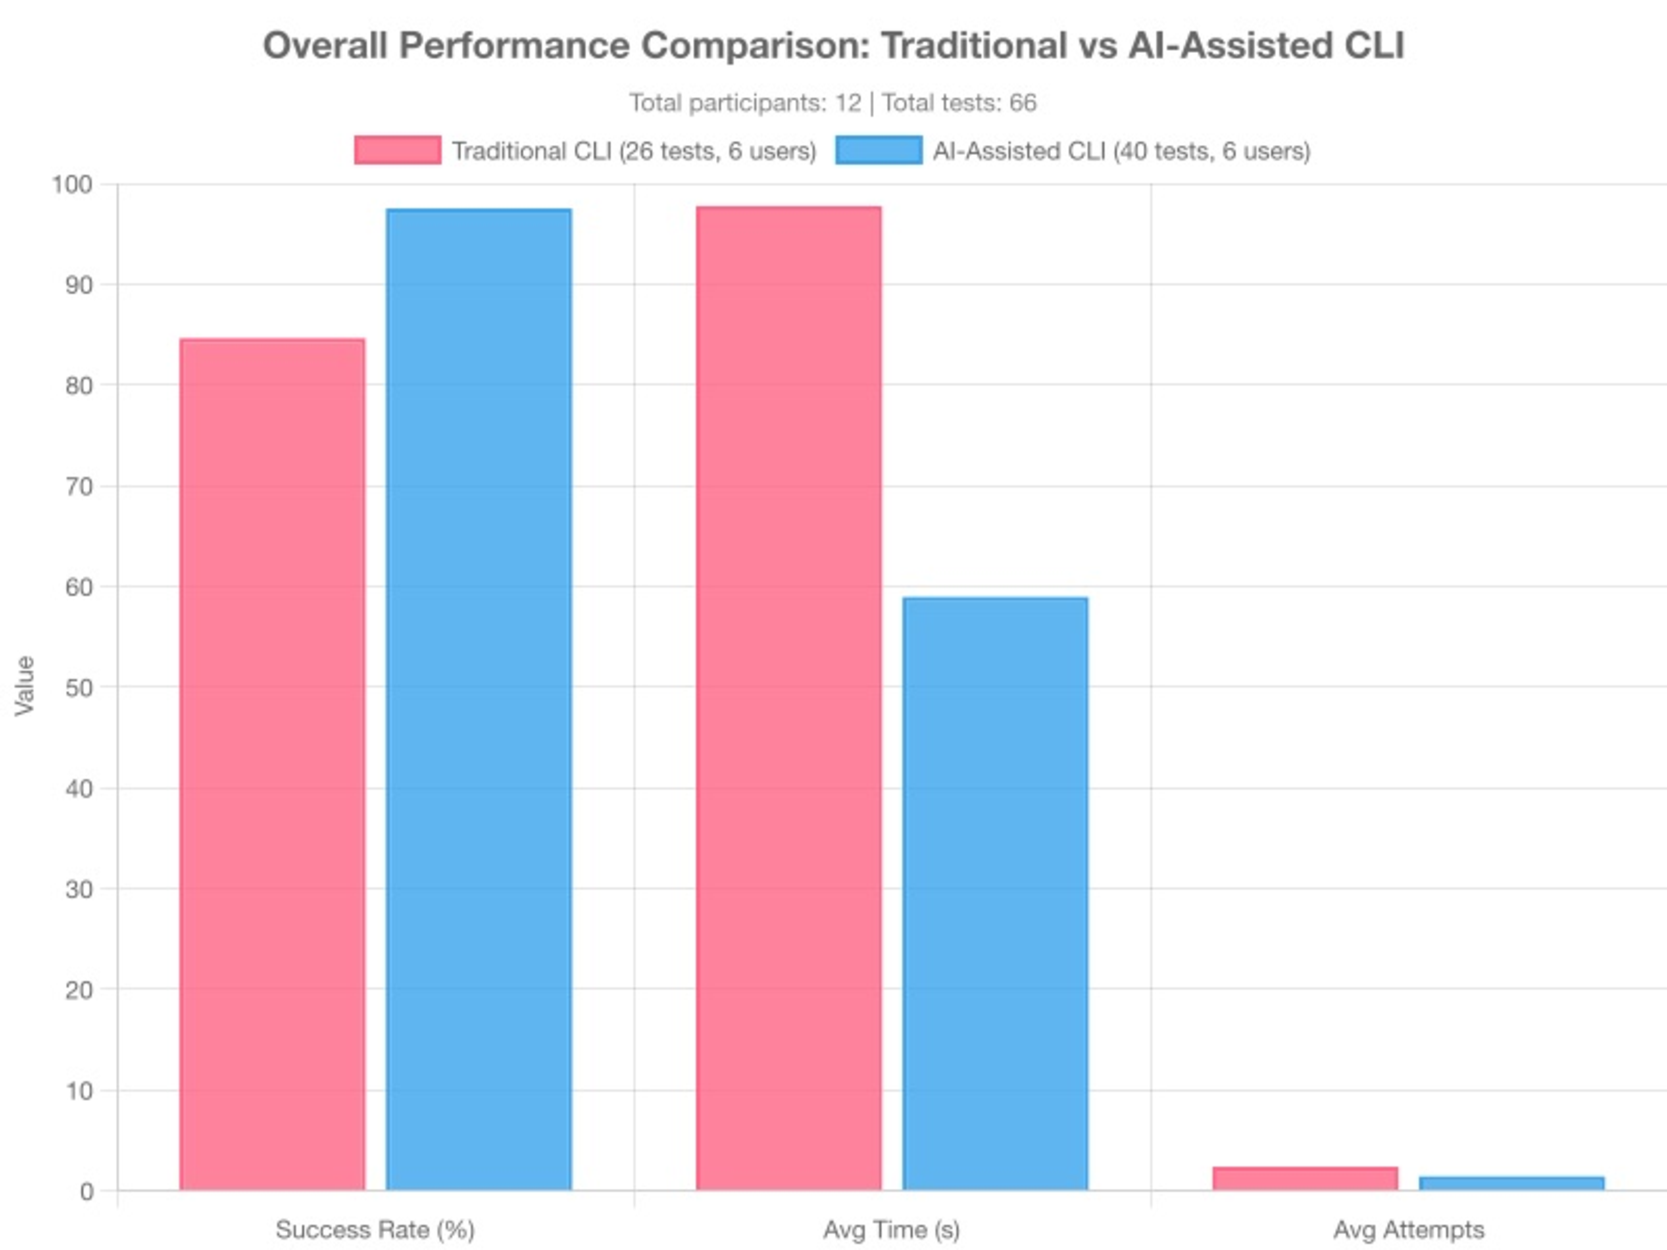
\includegraphics[width=0.8\textwidth]{assets/figures/performance_comparison.pdf}
	\caption{Overall Performance Comparison: Traditional vs AI-Assisted CLI}
	\label{fig:performance_comparison}
\end{figure}

\subsection{Success Rate and Attempt Metrics}

The success rate analysis shows that AI-assisted CLI achieved 97.5\% task completion success compared to 84.6\% for traditional CLI. The category-specific analysis reveals dramatic differences in task completion capability:

\begin{itemize}
	\item \textbf{Perfect AI performance:} File management (100\% vs 91.7\%), File navigation (100\% vs 100\%), File search (100\% vs 0\%), and Text processing (100\% vs 0\%)
	\item \textbf{Challenging categories:} File viewing (100\% vs 50\%) and Text search (80\% vs 0\%) show AI's effectiveness in complex syntax tasks
	\item \textbf{Traditional-only categories:} Disk usage (66.7\% success) and Process management (100\% success) were only attempted without AI assistance
\end{itemize}

Users required significantly fewer attempts to complete tasks successfully (1.43 vs 2.38 attempts on average), representing a 40\% reduction in trial-and-error behavior. Error analysis reveals that execution errors are the most common error type, occurring in 100\% of traditional CLI tests compared to 20\% with AI assistance. Incorrect command errors and task skipping were also substantially reduced with AI support.

Figure~\ref{fig:category_performance} shows the success rates across different task categories, highlighting the areas where AI assistance provides the most significant benefits.

\begin{figure}[h]
	\centering
	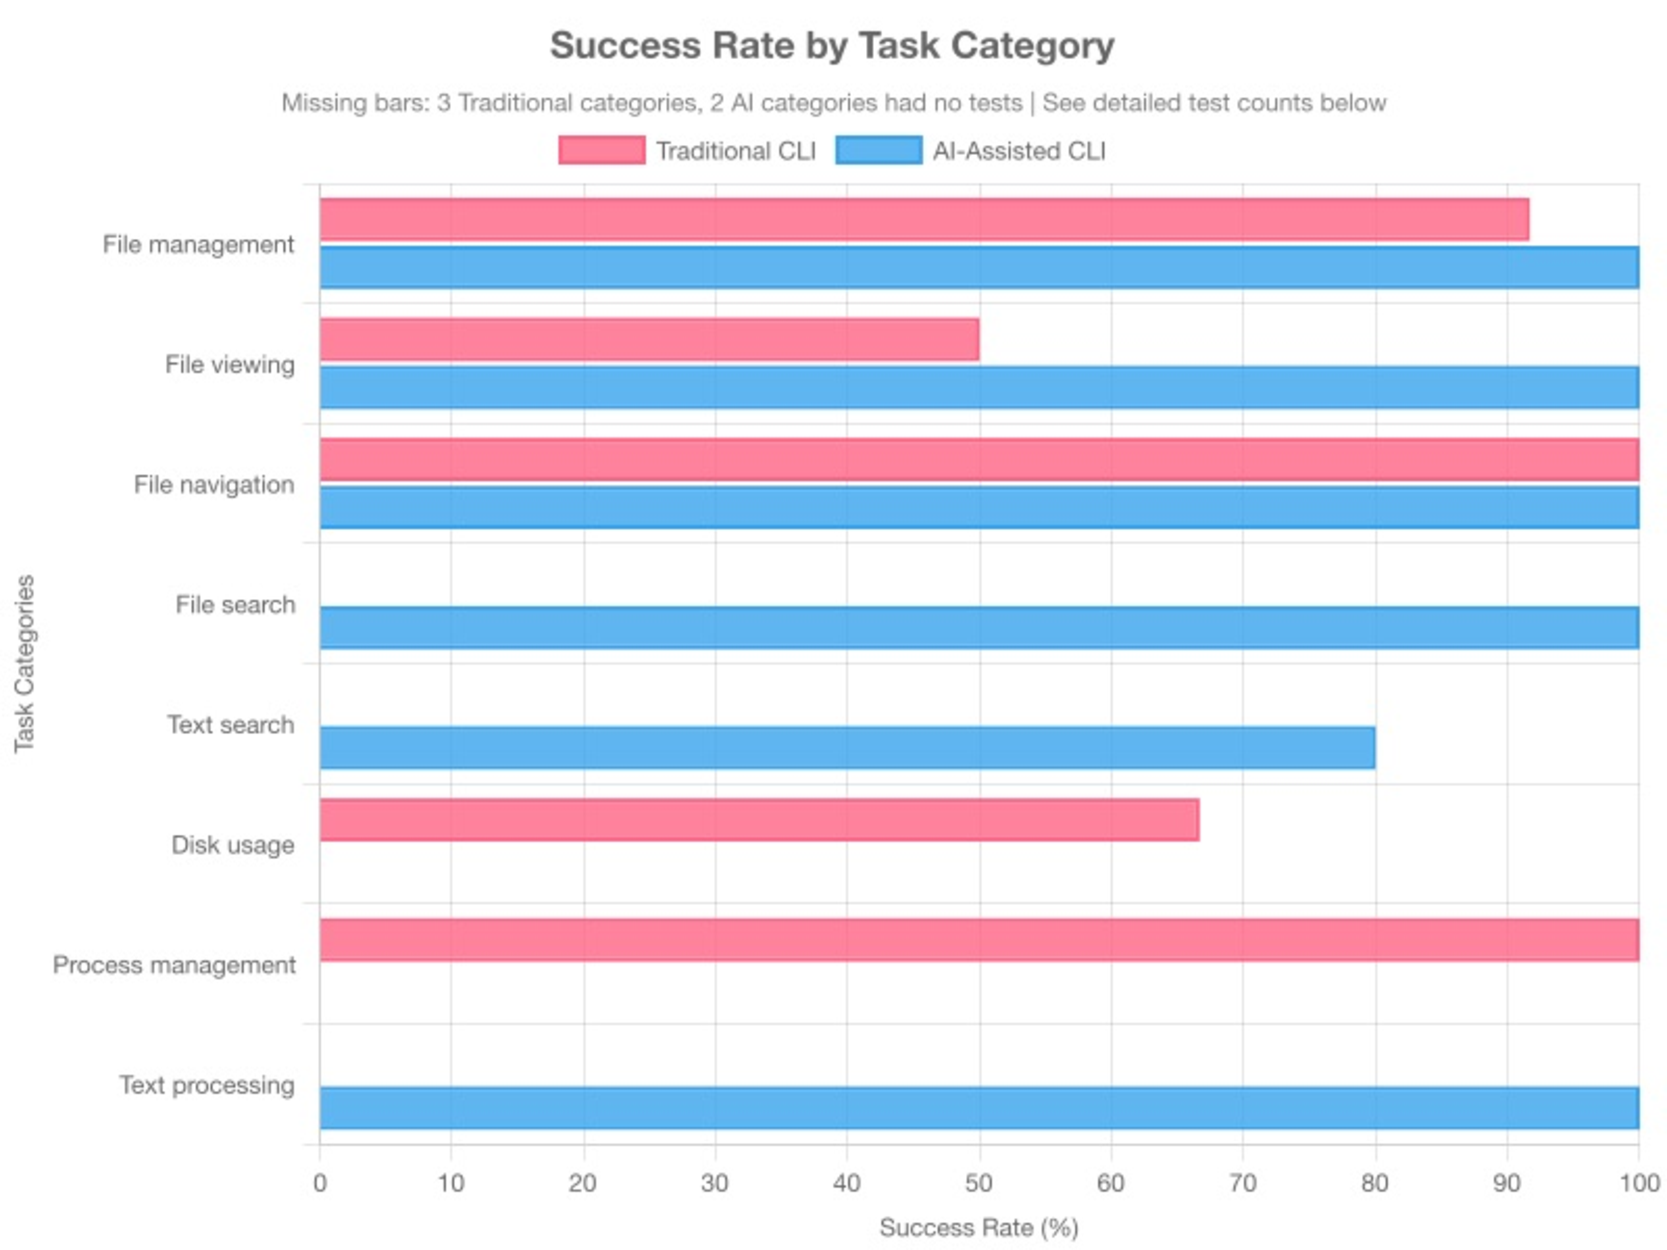
\includegraphics[width=0.9\textwidth]{assets/figures/category_performance_horizontal.pdf}
	\caption{Success Rate by Task Category}
	\label{fig:category_performance}
\end{figure}

Figure~\ref{fig:error_analysis} provides a detailed breakdown of error types and their frequencies across both interface conditions.

\begin{figure}[h]
	\centering
	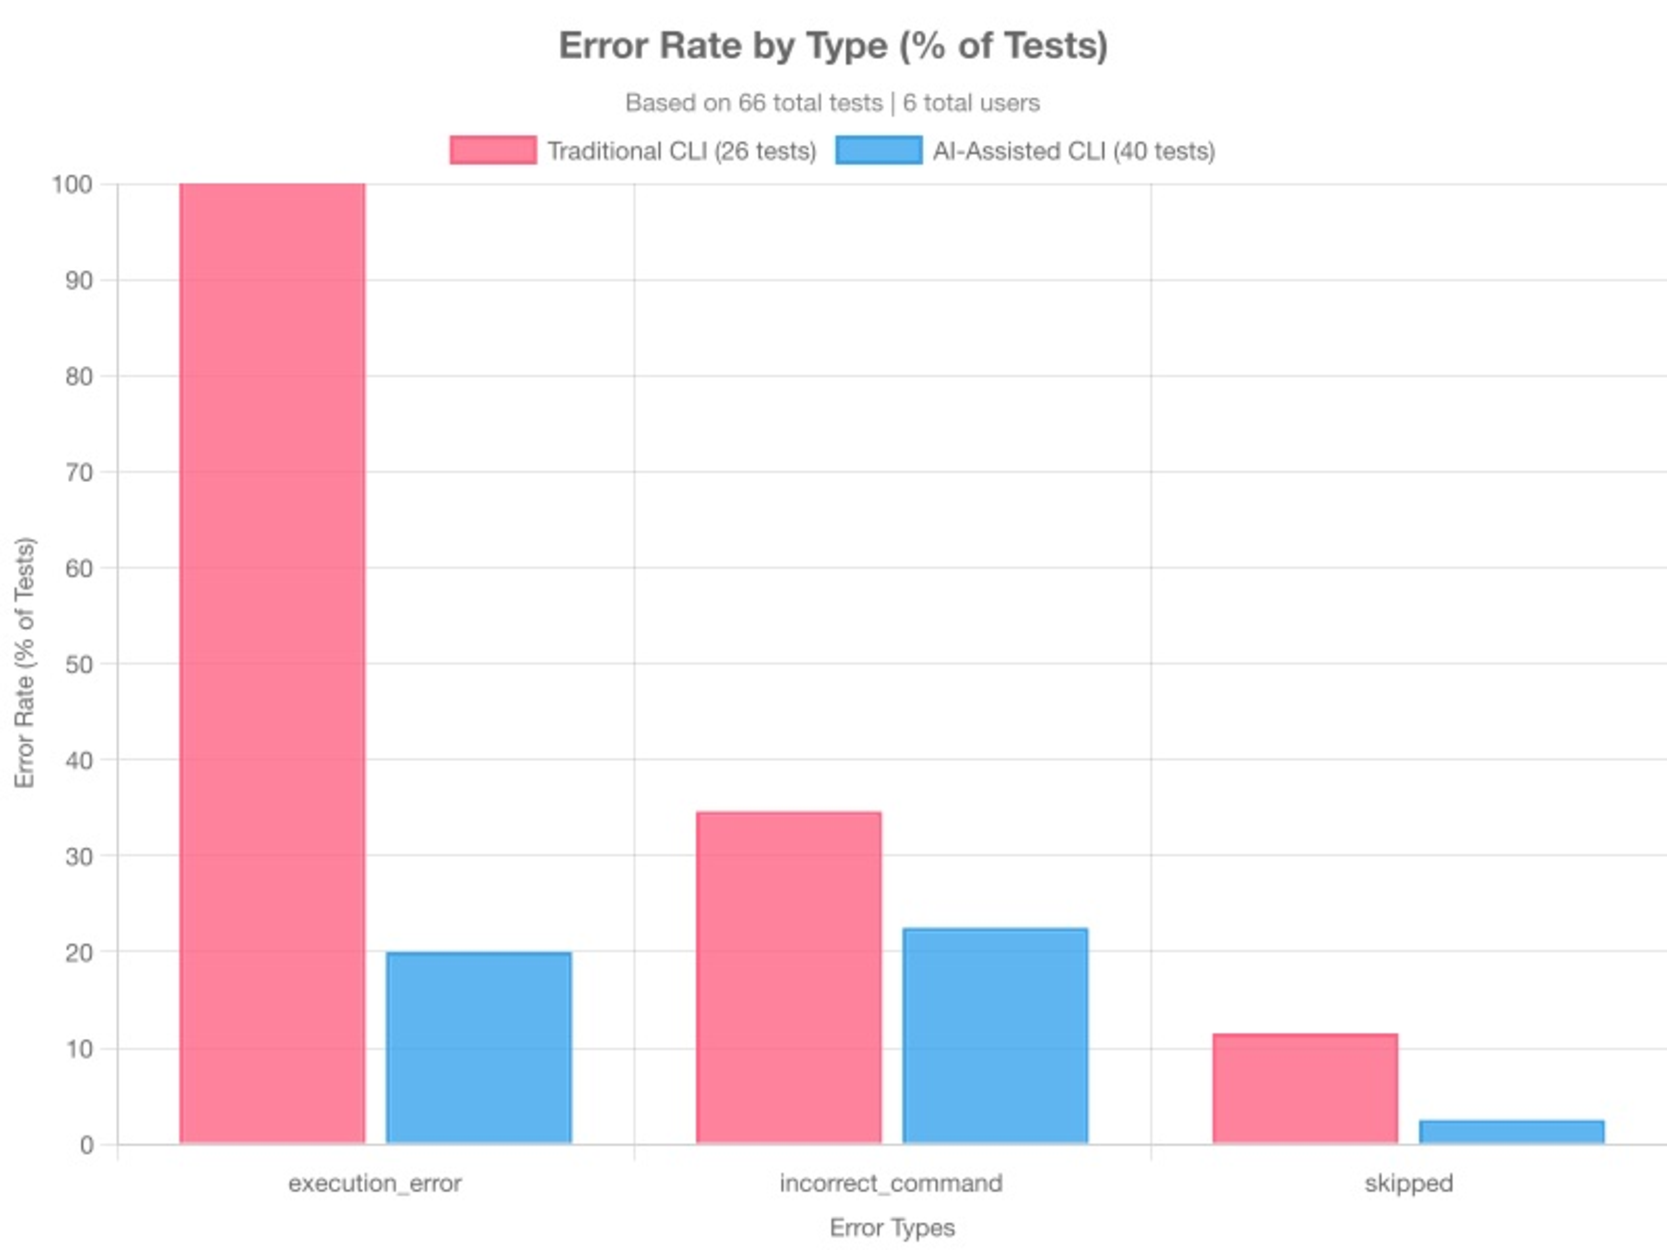
\includegraphics[width=0.8\textwidth]{assets/figures/error_analysis.pdf}
	\caption{Error Rate by Type (\% of Tests)}
	\label{fig:error_analysis}
\end{figure}

\section{Qualitative Feedback Analysis}

Beyond quantitative metrics, user feedback provides valuable insights into the subjective experience of using AI-assisted CLI tools. This qualitative data helps contextualize the numerical results and identifies areas for future improvement in AI-CLI design.

\subsection{User Satisfaction and Interface Preferences}

User satisfaction was measured across three dimensions using 5-point comparative scales. Results show strong preference for AI-assisted CLI across all satisfaction metrics:

\begin{itemize}
	\item \textbf{Ease of Use:} Average rating of 4.83/5, indicating users found AI-assisted CLI much easier to use than traditional CLI
	\item \textbf{Confidence:} Average rating of 3.83/5, showing users felt more confident with AI assistance available
	\item \textbf{Frustration:} Average rating of 2.17/5, indicating AI-assisted CLI was less frustrating to use (lower scores indicate less frustration)
\end{itemize}

These satisfaction ratings demonstrate that AI assistance not only improves objective performance metrics but also enhances the subjective user experience, making CLI interactions more accessible and less stressful for users.

Figure~\ref{fig:user_satisfaction} illustrates the user preference ratings across the three satisfaction dimensions.

\begin{figure}[h]
	\centering
	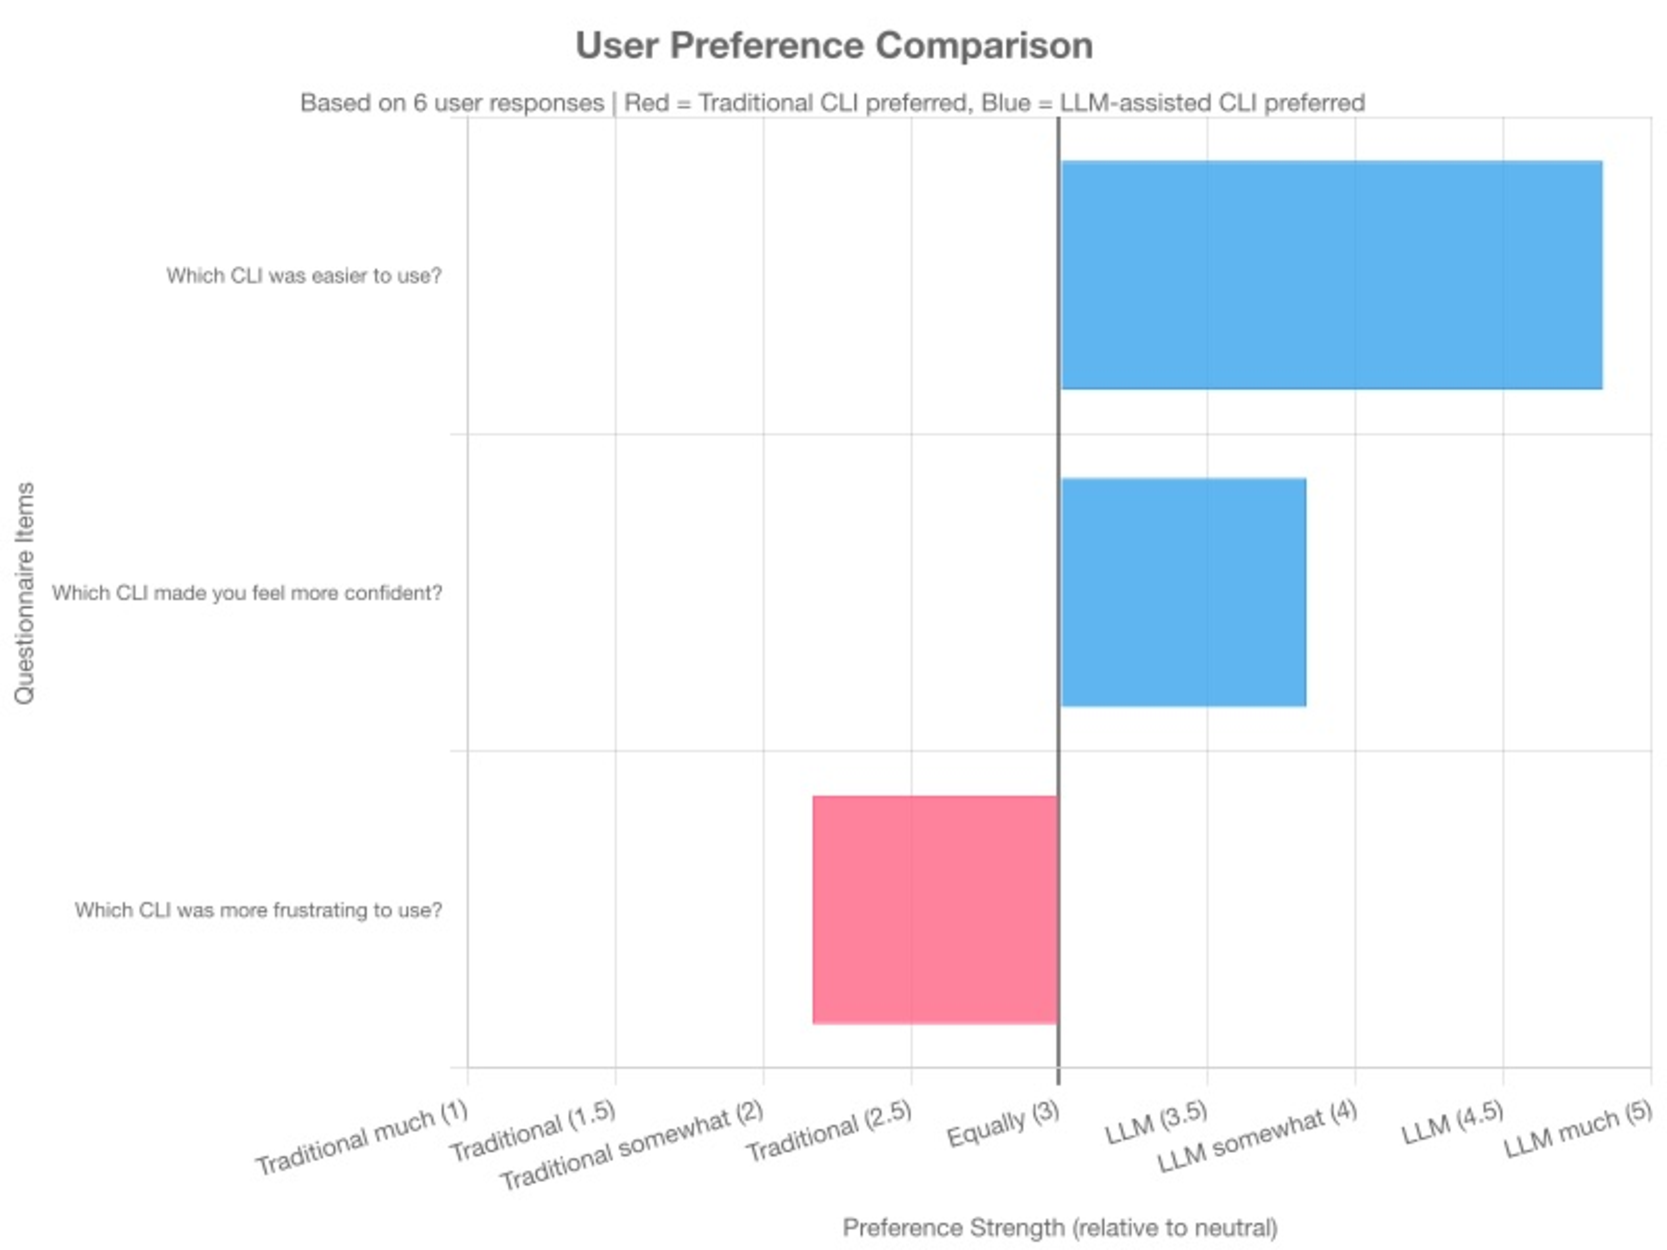
\includegraphics[width=0.9\textwidth]{assets/figures/user_satisfaction.pdf}
	\caption{User Preference Comparison}
	\label{fig:user_satisfaction}
\end{figure}

The study participants represented a diverse age distribution, as shown in Figure~\ref{fig:demographics_age}, ensuring that the results reflect a broad range of user experiences.

\begin{figure}[h]
	\centering
	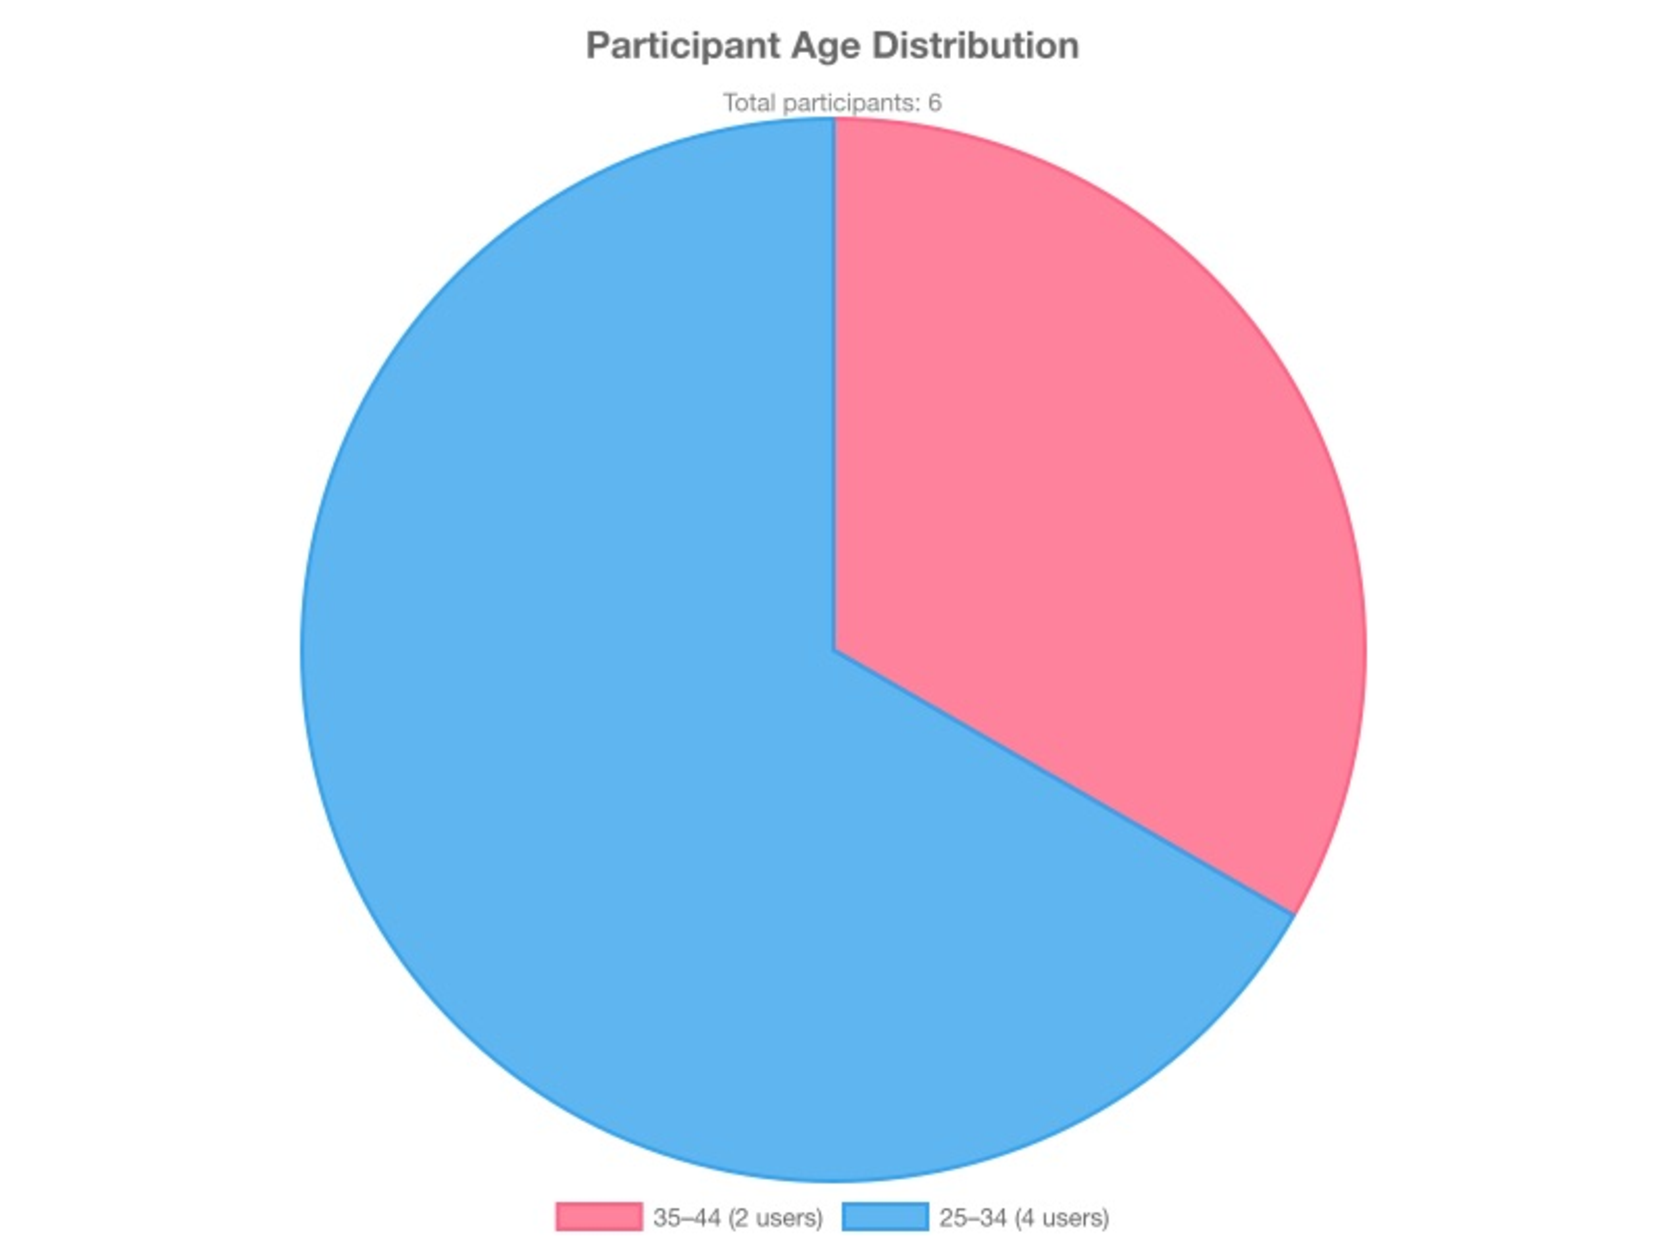
\includegraphics[width=0.7\textwidth]{assets/figures/demographics_age.pdf}
	\caption{Participant Age Distribution}
	\label{fig:demographics_age}
\end{figure}

\section{Comparative Analysis}

This section synthesizes the quantitative and qualitative findings to provide a comprehensive comparison between traditional and aiman systems. The analysis examines performance improvements and their implications for command-line interface usage.

\subsection{Performance Improvements by Task Category}

The experimental data reveals distinct patterns of AI effectiveness across different task categories, with some categories showing complete transformation while others demonstrate moderate improvements:

\textbf{Transformative Impact Categories:}
\begin{itemize}
	\item \textbf{File search and Text processing:} These categories were only successfully completed with AI assistance (0\% traditional success vs 100\% AI success), indicating AI's critical role in complex syntax operations
	\item \textbf{File viewing:} Showed the most dramatic time improvement (90\% reduction) and success rate improvement (50\% to 100\%)
\end{itemize}

\textbf{Moderate Improvement Categories:}
\begin{itemize}
	\item \textbf{File management:} Consistent improvements in both time (43\% faster) and success rate (91.7\% to 100\%)
	\item \textbf{File navigation:} Maintained perfect success rates while achieving 40\% time reduction
\end{itemize}

\textbf{Proficiency Correlation:} Analysis by CLI proficiency level shows that AI assistance benefits users across all skill levels, with intermediate users (level 3) showing the most consistent improvements. Higher proficiency users (level 4) still benefited from AI assistance, particularly in unfamiliar command domains.

Figure~\ref{fig:proficiency_correlation} demonstrates the relationship between CLI proficiency levels and success rates across both interface conditions.

\begin{figure}[h]
	\centering
	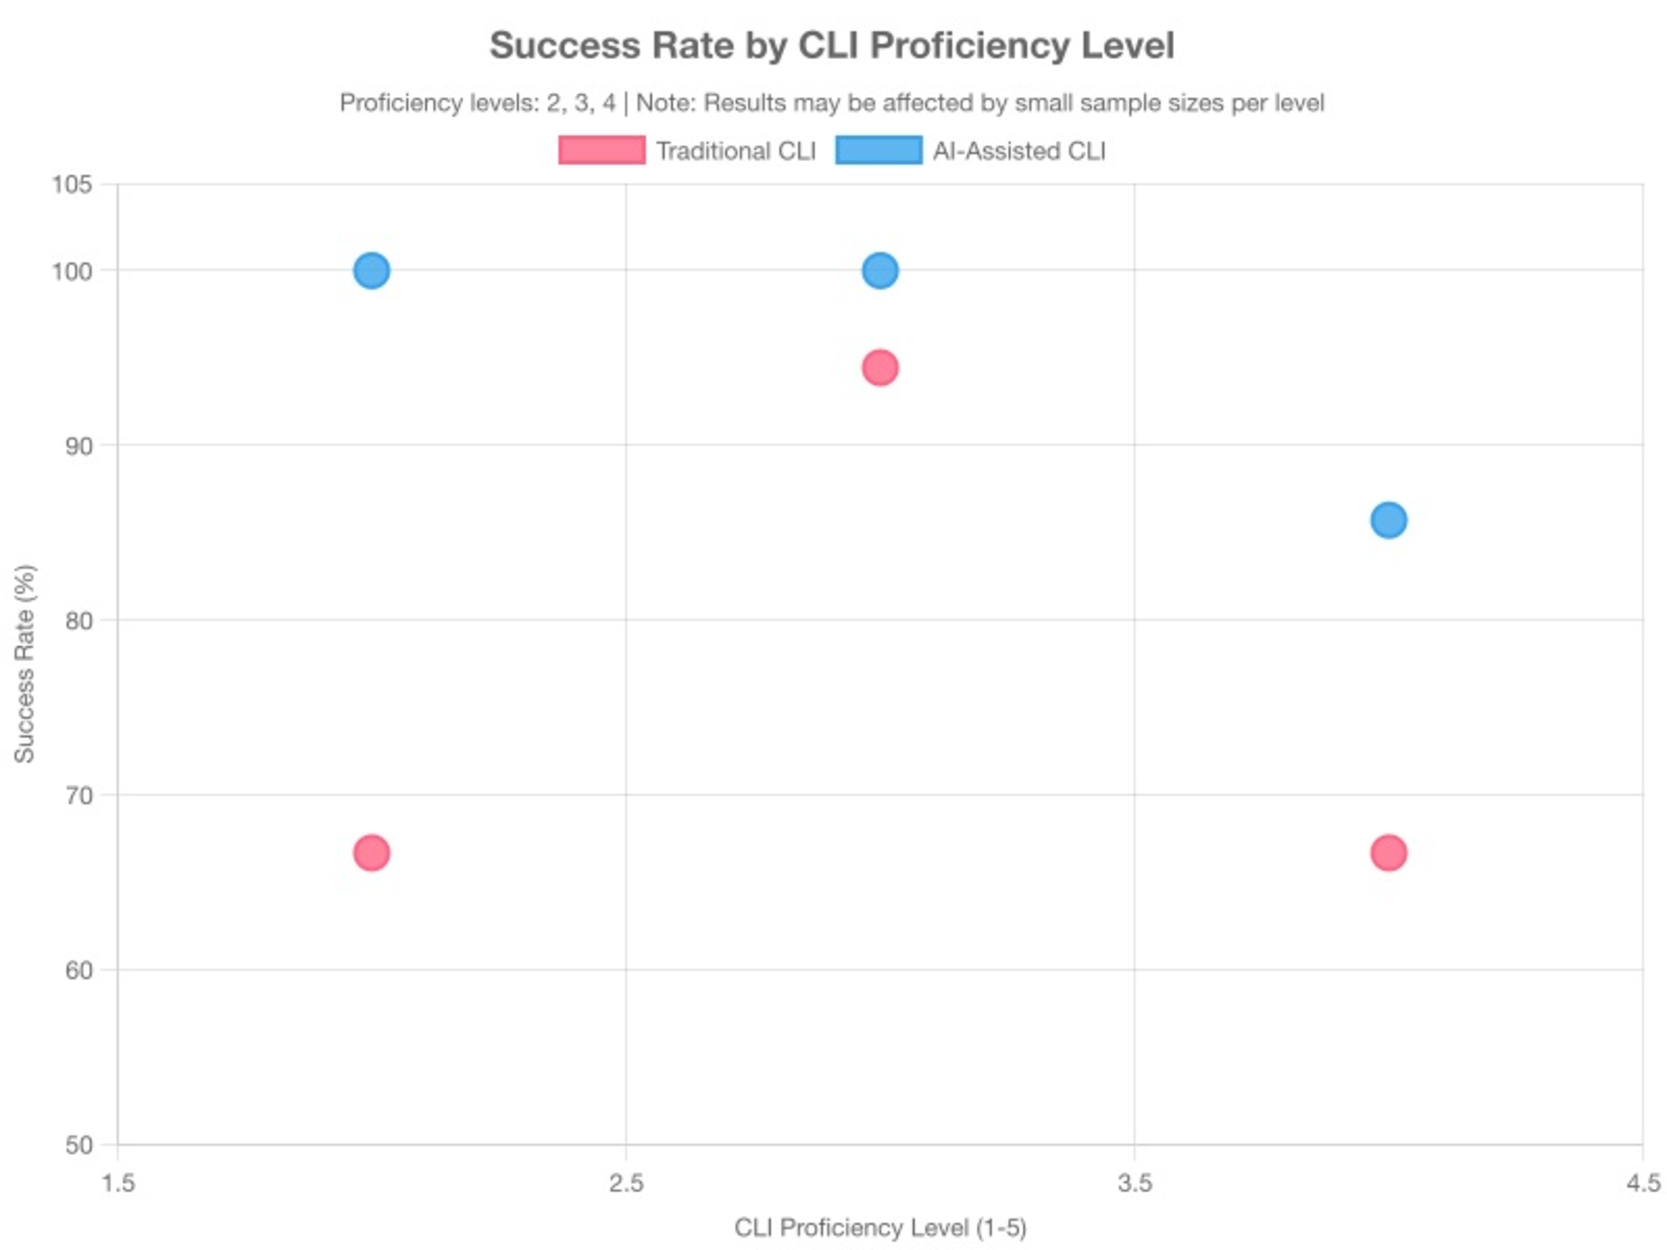
\includegraphics[width=0.8\textwidth]{assets/figures/proficiency_correlation.pdf}
	\caption{Success Rate by CLI Proficiency Level}
	\label{fig:proficiency_correlation}
\end{figure}

The time comparison analysis by task category, shown in Figure~\ref{fig:time_comparison}, reveals the specific areas where AI assistance provides the most substantial time savings.

\begin{figure}[h]
	\centering
	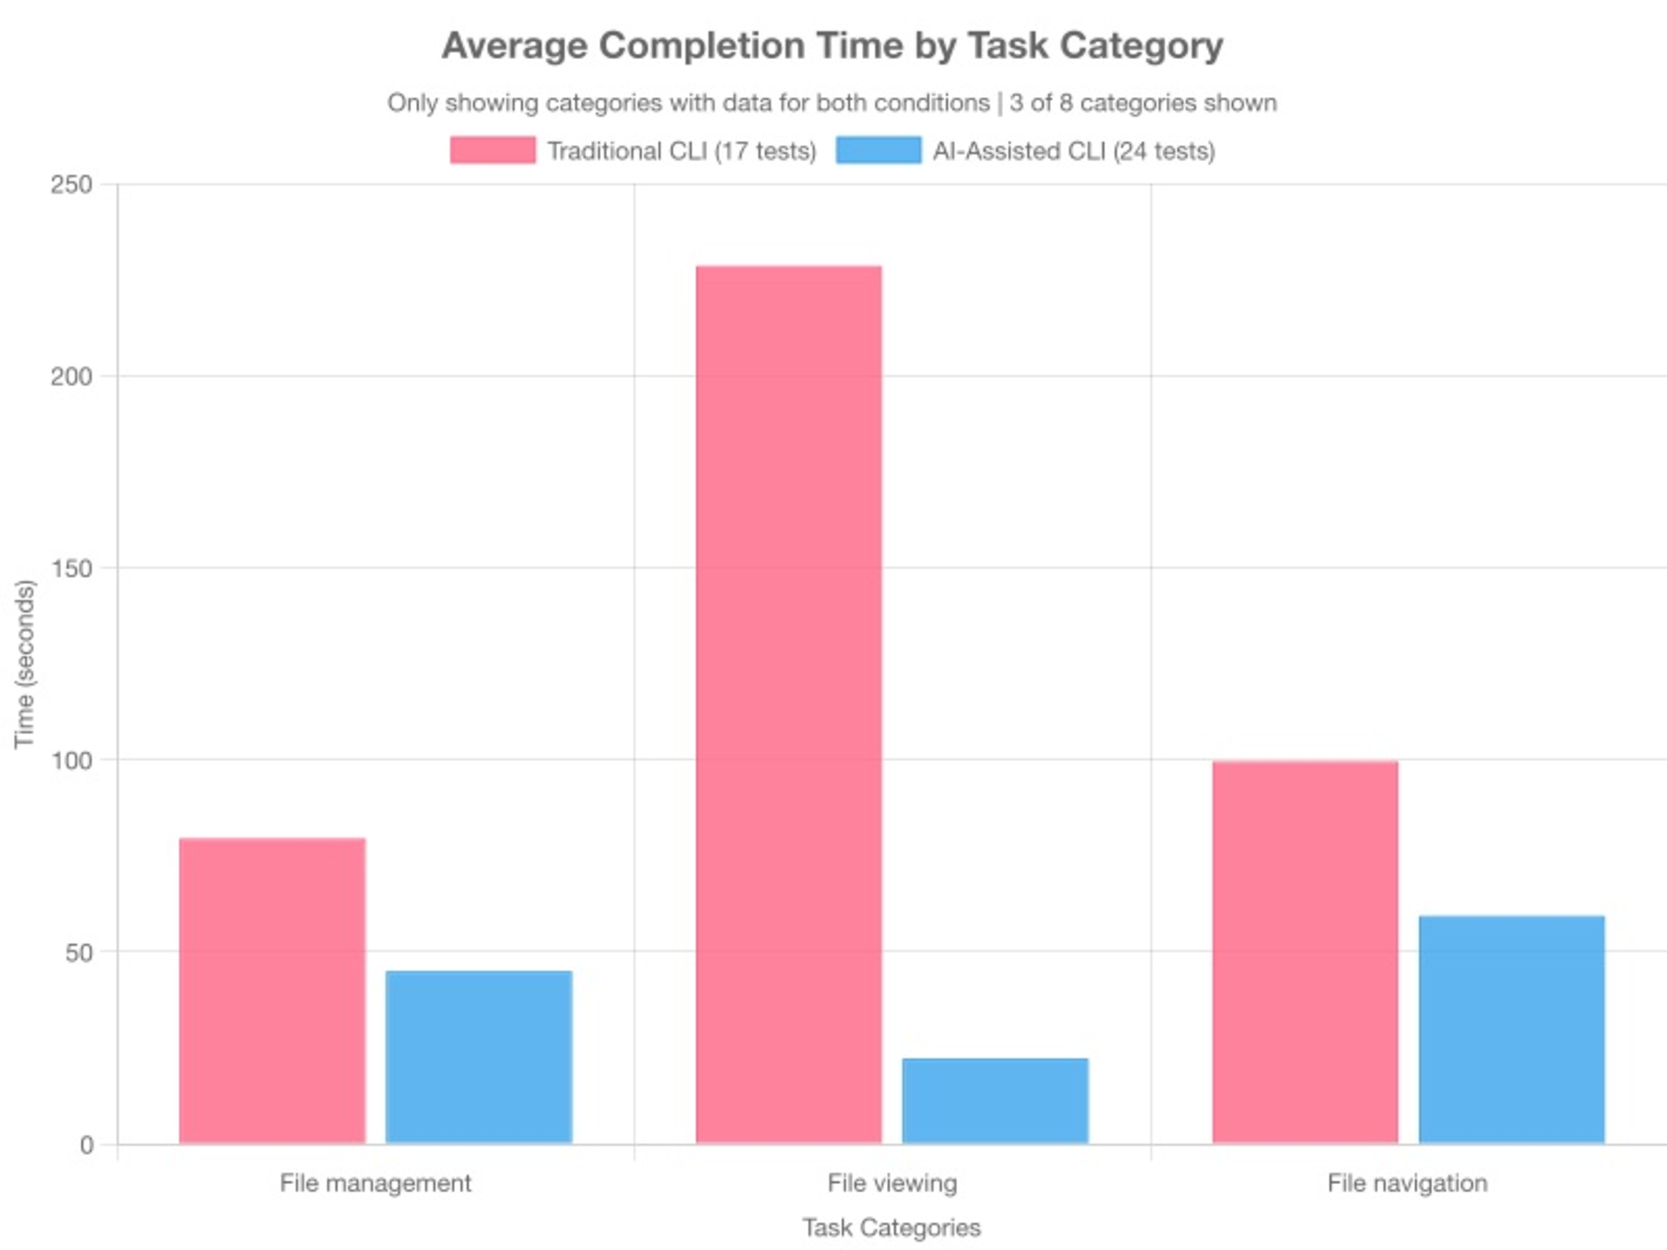
\includegraphics[width=0.9\textwidth]{assets/figures/time_comparison_by_category.pdf}
	\caption{Average Completion Time by Task Category}
	\label{fig:time_comparison}
\end{figure}

\subsection{Error Pattern Analysis}

The error analysis reveals significant differences in error types and frequencies between traditional and AI-assisted CLI usage:

\begin{itemize}
	\item \textbf{Execution errors:} The most common error type, reduced from 100\% occurrence rate in traditional CLI to 20\% with AI assistance
	\item \textbf{Incorrect commands:} Reduced from 35\% to 23\% occurrence rate, showing AI's effectiveness in syntax correction
	\item \textbf{Task skipping:} Dramatically reduced from 12\% to 3\%, indicating improved user confidence and task completion
\end{itemize}

The error reduction patterns align with the task category analysis, showing that AI assistance is most effective in preventing syntax-related errors and providing corrective guidance when commands fail. This contributes directly to the improved success rates and reduced attempt counts observed across all task categories.

